% Source: graduate-coursework/Sp26/CSCE775/Project/proposal_asv_3/proposal3_asv.tex
% Description: Hierarchical action space. The discrete mode selection (top) biases the interpretation of the 7 continuous parameters (bottom). Each mode defines characteristic operating ranges for heading, speed, and sensor duty-cycle ratios, though the continuous parameters allow fine-grained adaptation within each mode.

\documentclass[border=4pt]{standalone}
\usepackage{amsmath,amssymb}
\usepackage{pgfplots}
\usepackage{tikz}
\usepackage{xcolor}
\pgfplotsset{compat=1.18}
\usetikzlibrary{positioning, arrows.meta, shapes.geometric, fit, calc, backgrounds, patterns, decorations.pathreplacing}

\definecolor{Garnet}{HTML}{73000A}
\definecolor{Atlantic}{HTML}{466A9F}
\definecolor{Congaree}{HTML}{1F414D}
\definecolor{Horseshoe}{HTML}{65780B}
\definecolor{Rose}{HTML}{CC2E40}
\definecolor{Honeycomb}{HTML}{A49137}
\definecolor{Black90}{HTML}{363636}
\definecolor{Black70}{HTML}{5C5C5C}
\definecolor{Black50}{HTML}{A2A2A2}
\definecolor{Black30}{HTML}{C7C7C7}
\definecolor{Black10}{HTML}{ECECEC}
\definecolor{WarmGrey}{HTML}{676156}


\begin{document}
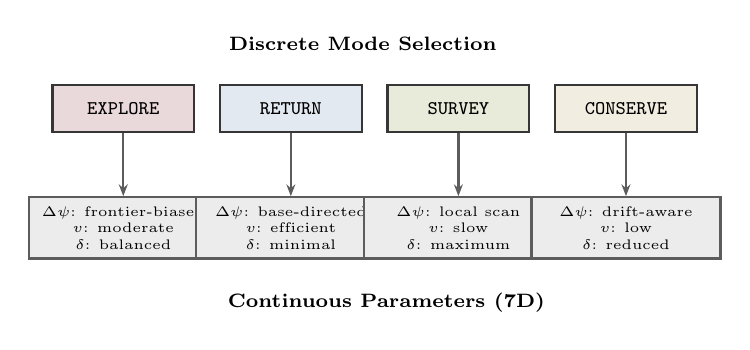
\begin{tikzpicture}[
    mode/.style={draw=Black90, thick, minimum width=1.8cm, minimum height=0.6cm, align=center, font=\scriptsize},
    param/.style={draw=Black70, thick, minimum width=2.4cm, minimum height=0.5cm, align=center, font=\tiny, fill=Black10},
    arr/.style={-{Stealth[length=1.5mm]}, thick, color=Black70},
    every node/.style={font=\scriptsize}
]

% Mode selection
\node[mode, fill=Garnet!15] (explore) {\texttt{EXPLORE}};
\node[mode, fill=Atlantic!15, right=0.3cm of explore] (return) {\texttt{RETURN}};
\node[mode, fill=Horseshoe!15, right=0.3cm of return] (survey) {\texttt{SURVEY}};
\node[mode, fill=Honeycomb!15, right=0.3cm of survey] (conserve) {\texttt{CONSERVE}};

\node[font=\scriptsize\bfseries, above=0.3cm of return.north east] {Discrete Mode Selection};

% Continuous params below each
\node[param, below=0.8cm of explore] (ep) {$\Delta\psi$: frontier-biased\\$v$: moderate\\$\delta$: balanced};
\node[param, below=0.8cm of return] (rp) {$\Delta\psi$: base-directed\\$v$: efficient\\$\delta$: minimal};
\node[param, below=0.8cm of survey] (sp) {$\Delta\psi$: local scan\\$v$: slow\\$\delta$: maximum};
\node[param, below=0.8cm of conserve] (cp) {$\Delta\psi$: drift-aware\\$v$: low\\$\delta$: reduced};

\draw[arr] (explore) -- (ep);
\draw[arr] (return) -- (rp);
\draw[arr] (survey) -- (sp);
\draw[arr] (conserve) -- (cp);

\node[font=\scriptsize\bfseries, below=0.3cm of rp.south east] {Continuous Parameters (7D)};

\end{tikzpicture}
\end{document}
